\newpage
\part{Implementation}

\newpage
\section{Implementation introduction}

% ML: ta kapitola je spis shrnuti zmen nez uvod :-) Ale uz to nech, tak jak to je
\subsection{pywps-demo}
During the implementation the \textit{pywps-demo}
(Sec. \ref{sub:demo}) running on \textit{Flask} framework was
used. This demo server instance runs on host machine server at port
5000 as well as the image built from its Dockerfile is used for every
container creation. For developing purpose some sections were added to
configuration file as well some minor changes for instance in server
routing were made. The diff file to pywps-demo is in
App. \ref{app:pywps-demo}.

\subsubsection{pywps-demo Dockerfile}
\textit{pywps-demo} is also available as a Dockerfile and as mentioned
the image built from this Dockerfile is used for container creation.
Before the work on this thesis started, the pywps-demo project had
offered two dockerfiles, both based on \textit{alpine Linux}
distribution. The first one \textit{pywps-flask} was the default
implementation using only Flask while the second one \textit{nginx}
implements pywps using Nginx and Green unicorn as WSGI server. During
the implementation only the \textit{pywps-flask} Dockerfile was
used. However it was necessary to modify the Dockerfile because it did
%% ML: je nekde vysvetleno, proc je potreba GDAL, pokud ano, tak zde chybi reference
not contain \textit{GDAL} library.

As a part of the work on this thesis new version of Dockerfile with
support of GDAL was created in collaboration with PyWPS
developers. There were some issues with \textit{Xerces} libraries
whose packages are not available for alpine distribution and its
manual instalation was necessary. The newly-created Dockerfile is
%% ML: ta posledni veta zni divne, v odstavci se opakuje casteji "work
%% on this thesis"
available in App. \ref{app:dockerfile}. At the end of the work on this
thesis pywps-demo offers dockerfiles based on \textit{alpine} and
\textit{ubuntu} Linux distribution.

\subsection{OWSLib}
A Python package \textit{OWSLib} was used for forwarding requests from
PyWPS server instance running on host machine to PyWPS server instance
%% ML: detailly?
running inside a Docker container. Some bug fixing which is detailly
described in Sec.\ref{sub:Container_execute} was necessary. Complete
%% ML: Byly ty upravy zacleneny do OWSlib, pokud ano, tak to zmin
diff is available in App. \ref{app:owslib}.

\subsection{PyWPS}
Most changes have been done in core PyWPS project. Almost all changes were made in \textit{processing} module. To this module new file
\textit{container.py} containing the \textit{Container} class was added. Complete diff is available at

\todo[inline]{Doplnit reference}

\newpage
\section{Operations overview}
\label{sec:operations_ov}
PyWPS in current version 4.0.0 implements all mandatory operations: \textit{Execute}, \textit{GetCapabilities}, \textit{DescribeProcess}.
Operations are handled by corresponding methods \textit{execute()}, \textit{get\_capabilities()} and \textit{describe()} in \textit{Service} class. 

However both \textit{GetCapabilities} and \textit{DescribeProcess}
operations run in synchronous mode only. After sending a request, a
client receives back GetCapabilities or DescribeProcess response (both
detaily described in \ref{para:GetCapa_response} and
\ref{para:DesribeProc_response}). Both operations return only
information or description about process but do not trigger the
execution of the process. It is supposed the response to
GetCapabilities and DescribeProcess is returned almost immediately.
During the GetCapabilities and the DescribeProcess operations a
process execution is not started and therefore there is no starting
%% ML: ta posledni veta zni divne
process to be isolated. That is why from this point on this thesis is
dedicated only to \textit{Execute} operation.

%% ML: chybi zdroj, pokud je to Tvuj diagram, tak to uved (napr. (source: author))
\begin{figure}[h!]
\centering
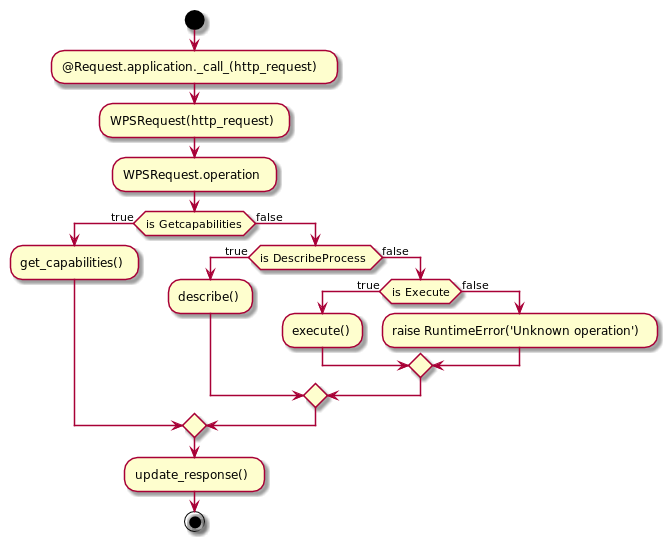
\includegraphics[width=0.9\textwidth]{img/Diag_operations.png}
\caption{PyWPS operations activity diagram}
\label{fig:Diag_operations}
\end{figure}

\section{Execute operation}
\subsection{Service.execute()}
As mentioned in previous section Sect. \ref{sec:operations_ov}, \textit{Execute} operation is handled by \textit{execute()} method.
Inputs for the method are:
\begin{itemize}
\item \textit{identifier} (string) - a name of the process which execution is requested and which is supported by WPS server.
\item \textit{wps\_request} (WPSRequest object) - an object containing original HTTP request.
\item \textit{uuid} (integer) - unique identifier of process execution.
\end{itemize}

%% ML: opet: zdroj
\begin{figure}[h!]
\centering
\begin{floatrow}
\ffigbox{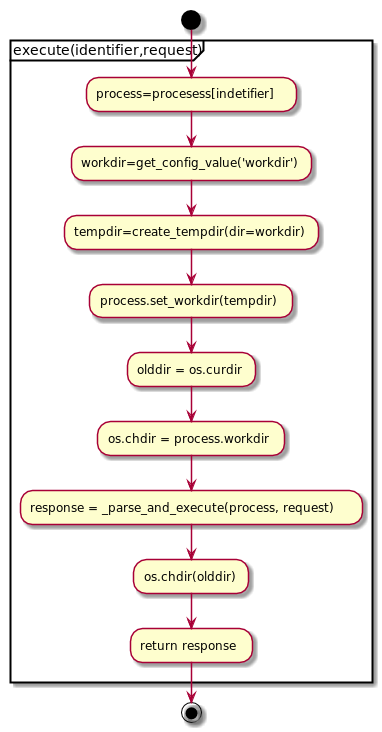
\includegraphics[width=0.4\textwidth]{img/Diag_service_execute.png}}{\caption{Activity diagram: method \textit{Service.execute()}}\label{fig:DiagServiceExecute}}
\ffigbox{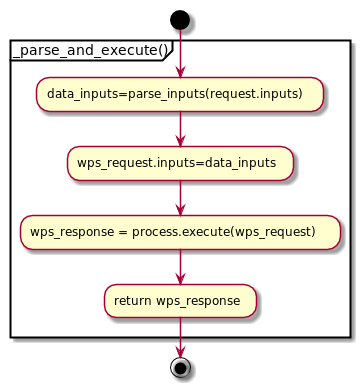
\includegraphics[width=0.4\textwidth]{img/Diag_service_parse_execute.png}}{\caption{Activity diagram: method \textit{Service.\_parse\_and\_execute()}}\label{fig:DiagServiceParseExecute}}
\end{floatrow}
\end{figure}

The flowchart of the process execution is displayed at Fig. \ref{fig:DiagServiceExecute}. 
At first a deepcopy of the process instance is created so that processes cannot override each other. Then a temporary working directory \textit{workdir} is created and set as a current workdir for the process execution. To the workdir all input files are
copied as well as all temporary files and outputs are stored here. Then the method \textit{\_parse\_and\_execute()} is called (see
Fig. \ref{fig:DiagServiceParseExecute}). Here the inputs are parsed, in case of web-referenced input, the data are downloaded to workdir, in case of directly in request sent data, the data are saved into a file in workdir. The process execution afterward runs in \textit{Process.execute()} method. This method returns a \textit{wps\_response} - an instance of \textit{WPSReponse} object.

\subsection{Process.execute()}
The method \textit{execute()} of class \textit{Process} contains crucial if-statement where is decided whether the process will be
run in asynchronous or synchronous mode. Running in asynchronous mode can be enforced by setting both attributes \textit{status} and \textit{storeExecuteResponse} of the \textit{ResponseDocument} element in the ExecuteRequest XML to True.

\bigskip
\begin{lstlisting}[basicstyle=\small,caption={ReponseForm element of ExecuteRequest XML},language=XML,label={lst:Execute_ResponseForm}]
<wps:ResponseForm>
 <wps:ResponseDocument status="true" storeExecuteResponse="true">
  <wps:Output asReference="true">
   <ows:Identifier>buff_out</ows:Identifier>
  </wps:Output>
 </wps:ResponseDocument>
</wps:ResponseForm>
\end{lstlisting}
\bigskip 

No matter whether the process runs synchronously or asynchronously always there is a control how many parallel processes are currently
running. The number of the maximum of concurrently running processes can be configured. If the process is asynchronous and the number of currently running processes exceeds the maximal number, the process is stored and its execution is started lately. In case of the synchronous process the \textit{ServerBusy} exception is raised. If the number of processes is smaller than the maximal number of 
concurrent processes, the process can be executed. In synchronous mode the \textit{\_run\_process()} is called, in asynchronous mode the method \textit{\_run\_async()} is called. The activity diagram of the \textit{Process.execute()} is displayed in Fig.\ref{fig:Diag_process_execute}.

%% ML: zdroj?
\begin{figure}[h!]
\centering
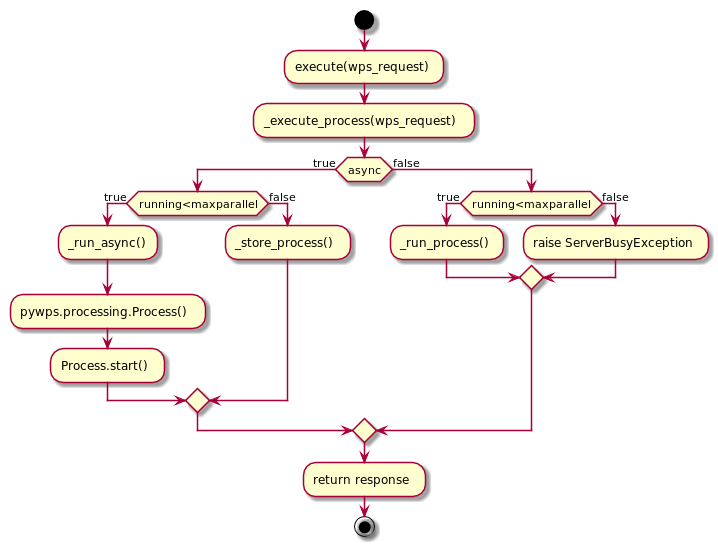
\includegraphics[width=0.9\textwidth]{img/Diag_process_execute.png}
\caption{\textit{Activity diagram: Process.execute()}}
\label{fig:Diag_process_execute}
\end{figure}

\subsection{Processing module}

%% ML: code -> operations ?
Until now the code described in this thesis was not
modified. Requirements which have been considered during the
implementation of Docker technology were that the source code will not
be very modified, the process isolation will be easily inserted and
the project structure will be kept the same. Keeping this in mind
changes in source code were made only in \textit{processing} module.

As mentioned in Sec. \ref{subsec:current_state}, PyWPS uses solely the Python package \textit{Multiprocessing} in production version.
In develop branch there is also \textit{Scheduler} extension as one of the option for multiprocessing. In this thesis another option 
\textit{Docker} for processing was added. The desired option for processing can be configured in configuration file via parameter \textit{mode} in section \textit{processing} (see Lst. \ref{lst:Mode_config}), possible values are:
\begin{itemize}
\item docker - new option
\item scheduler
\item multiprocessing - default option
\end{itemize}

\bigskip
\begin{lstlisting}[basicstyle=\small,caption={Processing mode configuration},language=XML,label={lst:Mode_config}]
[processing]
mode=docker/scheduler/multiprocessing
\end{lstlisting}

%% ML: zdroj
\begin{figure}[h!]
\centering
\begin{floatrow}
\ffigbox{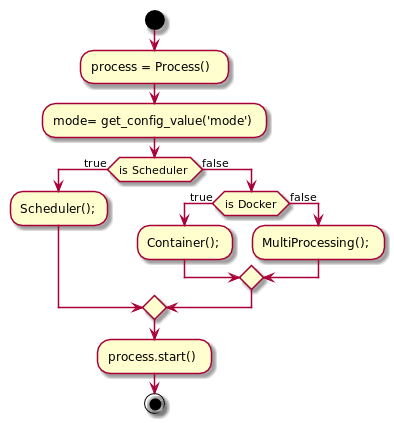
\includegraphics[width=0.48\textwidth]{img/Diag_run_async.png}}{\caption{Activity diagram: Method \textit{Process.\_run\_async() }}}{\label{fig:Diag_run_async}}
\ffigbox{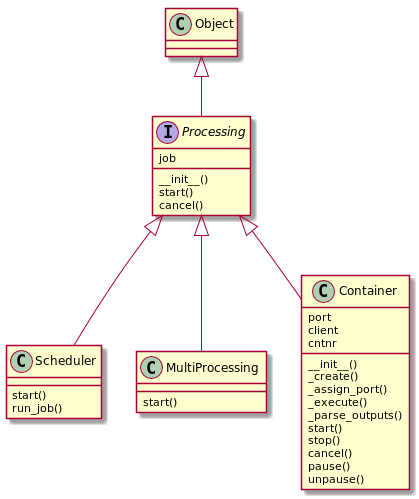
\includegraphics[width=0.48\textwidth]{img/Diag_class_processing.png}}{\caption{Class diagram: \textit{Processing} class}}{\label{fig:Diag_class_proc}}
\end{floatrow}
\end{figure}

\bigskip
The whole Docker implementation is in \textit{Container.py} module. The class \textit{Container} handles containers creation, interaction with
server, file-system mounting and all container management.

\newpage
\section{\textit{Container} class}
The main idea of process isolation using Docker is quite simple. For every process execution one separate Docker container is created.
Instead of starting process execution on the host PyWPS server after receiving ExecuteRequest from the client, the ExecuteRequest is
forwarded to PyWPS server running inside Docker container. The process execution runs inside the container. After successful process
execution the outputs are available at the host server. The host server and the container share the same process workdir at filesystem.

%% ML: zdroj
\bigskip
\begin{figure}[h!]
\centering
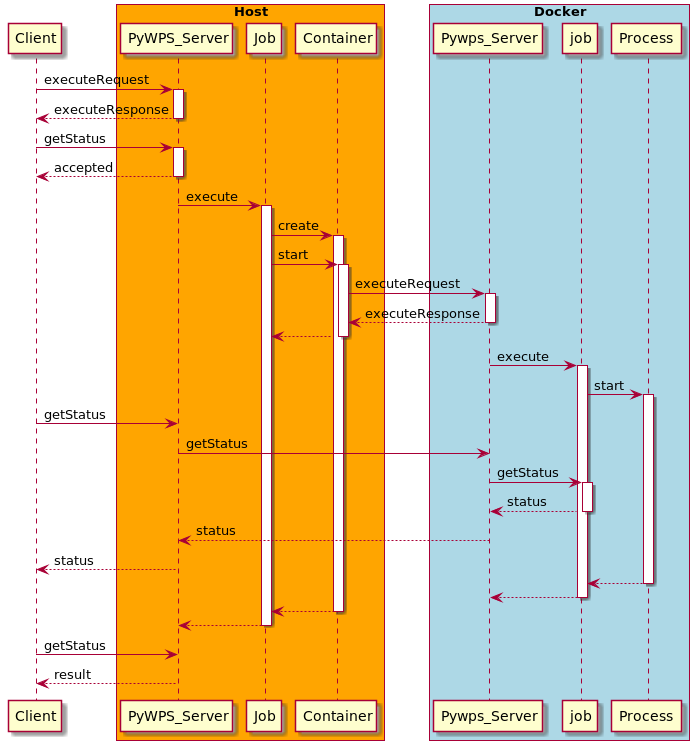
\includegraphics[width=0.9\textwidth]{img/Diag_sequence.png}
\caption{Sequence diagram: Process execution using Docker}
\label{fig:Diag_sequence}
\end{figure}

\subsection{\textit{Container} class constructor}
\label{sub:Container_init}

%% ML: opravit preteceni textu
\textit{Container} class is initialized with standard Python method
\textit{\_\_init\_\_()}. As an inheritor of \textit{Processing} class,
at first the parent constructor is called with
\textit{super().\_\_init\_\_()} method. Follows description of methods
which are called inside the constructor method.

\bigskip
\begin{lstlisting}[basicstyle=\small,caption={\textit{Container} class constructor},label={lst:Container_constructor}]
def __init__(self, process, wps_request, wps_response):
    super().__init__(process, wps_request, wps_response)
    self.port = self._assign_port()
    self.client = docker.from_env()
    self.cntnr = self._create()
\end{lstlisting}

\subsubsection{\textit{Container.\_assign\_port()}}
The method returns the number of available port. The port is chosen from range <\textit{port\_min},
\textit{port\_max}> which are both configurable values. If no port from the range is available, the method returns
\textit{NoAvailablePortException}. Schema of ports assignment to each container is in Fig. \ref{fig:Diag_port}.

\subsubsection{\textit{docker.from\_env()}} The \textit{docker} is a Python library for the Docker Engine API. \textit{from\_env} method
returns an instance of \textit{DockerClient} class which is a client to communicate with the Docker daemon. The returned client is
configured from the same variables as the Docker command-line client.

\subsubsection{\textit{Container.\_create()}} The \textit{\_create} method reads following values at the beginning:
\begin{itemize}
\item \textit{cntnr\_img} - Name of the image the container will be created from. The name of the image must be the same as the tag
set by the \textit{-t} parameter in \textit{docker build} command when the image is built from Dockerfile.

\bigskip
\begin{lstlisting}[basicstyle=\small,caption={Docker build command}]
docker build -t image_name /path/to/dockerfile
\end{lstlisting}

\item \textit{prcs\_inp\_dir} - Path to process workdir from \textit{self.job.wps\_response.process.workdir}. It is a directory where the
inputs for the process are stored.
\item \textit{prcs\_out\_dir} - Path to server output directory where all outputs are stored. The path is taken from \textit{outputpath}
parameter of section \textit{server} in the configuration file.
\item \textit{dckr\_inp\_dir} - Path to input data directory of WPS instance running inside Docker container. It is taken from 
\textit{dckr\_inp\_dir} of \textit{processing} section.
\item \textit{dckr\_out\_dir} - Path to output directory of WPS instance running inside the container. It is taken from 
\textit{dckr\_out\_dir} of \textit{processing} section.
\end{itemize}

The method returns an instance of \textit{Container} class from \textit{docker} module. The container is created by
\textit{self.client.containers.create()} method. 

The method takes optional parameter \textit{ports}. It is a dictionary
to define ports to bind inside the container. The keys of the
dictionary are the ports to bind inside the container (port 5000
inside \textit{Container 1} and \textit{Container 2} at
Fig. \ref{fig:Diag_port}). The values of the dictionary are the
corresponding ports to open on the host (port 5050 for \textit{Job1},
port 5051 for \textit{Job2} at Fig. \ref{fig:Diag_port}).

\begin{figure}[h!]
\centering
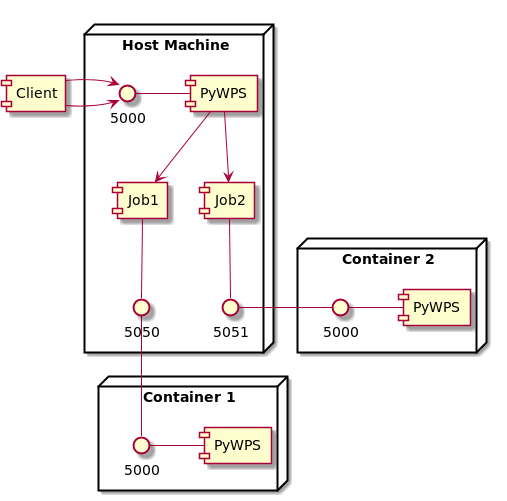
\includegraphics[width=0.55\textwidth]{img/Diag_ports.png}
\caption{Ports assignment schema}
\label{fig:Diag_port}
\end{figure}

Another optional parameter is \textit{volumes}. It is a dictionary 
to configure volumes mounted inside the container. The key is the host path and the value is a dictionary with the keys: \textit{bind}
- the path to mount the volume inside the container, and \textit{mode} - either \textit{rw} to mount the volume read/write, or 
\textit{ro} to mount it read-only.

%% ML: zdroj
\bigskip
\begin{lstlisting}[basicstyle=\small,caption={\textit{create()} method}]
self.client.containers.create(cntnr_img, detach=True,
ports={"5000/tcp": self.port}, 
volumes={prcs_out_dir: {'bind': dckr_out_dir, 'mode': 'rw'},
         prcs_inp_dir: {'bind': dckr_inp_dir, 'mode': 'ro'}})
\end{lstlisting}

Every container created with defined parameters \textit{volumes} and
\textit{ports} will have output directory on the host mounted into the
container output directory as well as the process workdir at host
machine mounted into container directory with data. Therefore, all
inputs downloaded to process workdir will be available for the
container and all outputs produced after process execution will be
%% ML: Shown?
stored at host machine output directory. Displayed in
Fig. \ref{fig:Diag_mount}.

%% ML: zdroj
\begin{figure}[h!]
\centering
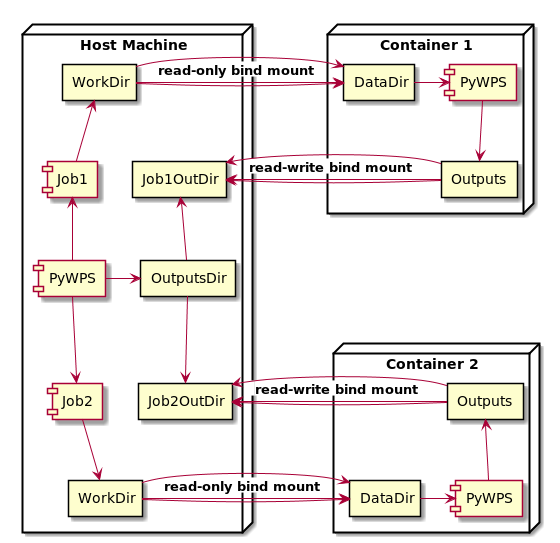
\includegraphics[width=0.65\textwidth]{img/Diag_mount.png}
\caption{Schema of mounting directories}
\label{fig:Diag_mount}
\end{figure}

%% ML: cela kapitola 9.2 neni uplne ctiva a prehledna (mozna by pomohl
%% opet nejaky diagram), zkus to jeste jednou projit, na velke upravy
%% ale neni cas
\subsection{\textit{Container.start()} method}
When a container is created the \textit{start()} method is called and the container is started.
In the time of finishing this thesis the method looks like at Lst.\ref{lst:Container_start}. In the current state is used the method
\textit{\_dirty\_clean()}. It assures that the container is removed after the successful execution, temporary workdir is cleaned and it also 
updates the process status in the database. Unfortunately, it causes that the process runs synchronously. To solve this problem is one of the
future goals.

%% ML: pokud bys mel ukazku kodu ocislovanou, mohl bys cisla radku
%% pouzivat jako referenci v dalsim textu
\begin{lstlisting}[basicstyle=\small,caption={\textit{Container.create()} method},label={lst:Container_start}]
def start(self):
    self.cntnr.start()
    time.sleep(0.5)
    self._execute()
    self._parse_status()
    self._dirty_clean()
\end{lstlisting}

\subsubsection{\textit{docker.container.start()}}
\textit{start()} method of \textit{Container} class from Python module \textit{docker}. The method is similar to \textit{docker start} command. 
It starts the Docker container. Then the method \textit{time.sleep()} is called to wait half a second after which the container is ready to 
use.

\subsubsection{\textit{Container.\_execute()}}
\label{sub:Container_execute}
\textit{\_execute()} method handles forwarding execution from server
to container. For sending request to container \textit{OWSLib}
%% ML: misto poznamky pod carou uved odkaz na kapitolu
library\footnote{\url{https://github.com/geopython/OWSLib}} is used.

\paragraph{OWSLib} is a Python package for client programming with OGC web services interface standards. However before it was possible
to use this package there was necessary to fix a bug in the \textit{wps} module. The bug caused outputs in the Execute response, which
were referenced as web-accesible resource, not to be parsed because of wrong handling with \textit{xlink} namespace. The bug-fix diff file 
is available in App. \ref{app:owslib}. 

\begin{lstlisting}[basicstyle=\small,caption={\textit{Container.\_execute()} method},label={lst:Container._execute}]
def _execute(self):
    url_execute = "http://localhost:{}/wps".format(self.port)
    inputs = get_inputs(self.job.wps_request.inputs)
    output = get_output(self.job.wps_request.outputs)
    wps = WPS(url=url_execute, skip_caps=True)
    self.execution = wps.execute(self.job.wps_request.identifier,
                                 inputs=inputs, output=output)
\end{lstlisting}

The method calls \textit{get\_inputs()} that 
returns all inputs transformed into a list of tuples in form \textit{(input\_name, input\_value)}. In case of ComplexData input, the input value is replaced with path to file. It is necessary to transform the inputs into the list of tuples because it is the required form for
\textit{WebProcessingService.execute()} method. Example for demo process \textit{buffer} at Lst. \ref{lst:Container.get_inputs}.

\begin{lstlisting}[basicstyle=\small,caption={\textit{get\_inputs} return value},label={lst:Container.get_inputs}]
the_inputs = [('poly_in', 'file:///pywps-flask/data/point.gml'),
              ('buffer', '1.0')]
the_outputs = [('buff_out', 'true')]
\end{lstlisting}

Then the method calls \textit{get\_outputs()} that returns list of tuples in form \textit{(output\_name, asReference\_attr\_value)}. It is 
necessary to transform the outputs into the list of tuples because it is the required form for \textit{WebProcessingService.execute()} method. 

\textit{WebProcessingService} object from OWSLib package is responsible for sending request to container. Its constructor takes URL of the
WPS server running inside container. Container URL varies depending on the port assigned to the container. Then the \textit{WPSExecution}
object is assigned to the \textit{Container} instance. The WPS\-Execution object is returned from \textit{WebProcessingService.execute()} 
method that takes as inputs process identifier, list of inputs from \textit{get\_inputs()} and outputs from \textit{get\_outputs()}.

\subsubsection{\textit{Container.\_parse\_status()}}
The method takes path to status location from \textit{WPSExecution.statusLocation} and copies it to \textit{Job.process.status\_url}.
Then the \textit{WPSReponse} object is updated by \textit{Job.wps\_response.update\_status()} with \textit{WPSExecution.statusMessage}.
It means the \textit{WPSResponse} object at host machine WPS server adopts \textit{statusMessage} and path to \textit{statusLocation}
from \textit{WPSExecution} object that handles the process execution inside the container. The process execution inside the container
updates its status into the file that is located in container output directory. This directory is shared with WPS server at host machine
si it is available even for the client.

\subsubsection{\textit{Container.\_dirty\_clean()}}
The method cares about stopping and removing Docker container, removing job workdir and original status XML. This method prevents to
accumulation of running Docker containers and temporary files in workdir directory. On the other hand there is missing functionality
for the process managment in database. In the current state when using Docker, the processes on the server are not ended even though
the result is already returned from the container. These pseudo-running processes accumulate on the server and some other processes
can be rejected because the limit of maximal running  processes is reached. This must be solved in the future.

\begin{lstlisting}[basicstyle=\small,caption={\textit{get\_inputs} return value},label={lst:Container.get_inputs}]
def _dirty_clean(self):
    time.sleep(1)
    self.cntnr.stop()
    self.cntnr.remove()
    self.job.process.clean()
    os.remove(self.job.process.status_location)
\end{lstlisting}

\textit{time.sleep(1)} is called to wait one second so the running process execution inside the container can be finished. The parameter
1 second is hardcoded and serves just now when the development is not done. \textit{stop()} and \textit{remove()} methods of class 
\textit{Container} from \textit{docker} module are similar to docker commands \textit{docker stop container\_id} and 
\textit{docker rm container\_id}.

\textit{Job.process.clean()} remove the job workdir so the temporary files do not cumulate at the server. \textit{os.remove()} deletes
the original status XML since the status XML from the container was sent back to the client.
